% !TeX program = xelatex
% !TeX encoding = UTF-8
% !TeX spellcheck = en_US
% !BIB program = biber
%% 
%%%%%%%%%%%%%%%%%%%%%%%%%%%%%%%%%%%%%%%%%%%%%%%%%%%%%%%%%%%%%%%%%%%%%%%%%%%%%%%%

%%%%%%%%%%%%%%%%%%%%%%%%%%%%%%%%%%%%%%%%%%%%%%%%%%%%%%%%%%%%%%%%%%%%%%%%%%%%%%%%
%% 
%%            JJJJ   K                         K   UUUU         UUUU  
%%            JJJJ   KKKK                   KKKK   UUUU         UUUU  
%%            JJJJ   KKKKKK               KKKKKK   UUUU         UUUU  
%%            JJJJ      KKKKKK         KKKKKK      UUUU         UUUU  
%%            JJJJ         KKKKKK   KKKKKK         UUUU         UUUU  
%%            JJJJ            KKKKKKKKK            UUUU         UUUU  
%%    JJ     JJJJJ               KKK               UUUUU       UUUUU  
%%  JJJJJJJJJJJJJ    KKKKKKKKKKKKKKKKKKKKKKKKKKK    UUUUUUUUUUUUUUU   
%%    JJJJJJJJJ      KKKKKKKKKKKKKKKKKKKKKKKKKKK      UUUUUUUUUUU     
%% 
%%             Template created by Michael Roland (2021)
%% 
%%%%%%%%%%%%%%%%%%%%%%%%%%%%%%%%%%%%%%%%%%%%%%%%%%%%%%%%%%%%%%%%%%%%%%%%%%%%%%%%

%%%%%%%%%%%%%%%%%%%%%%%%%%%%%%%%%%%%%%%%%%%%%%%%%%%%%%%%%%%%%%%%%%%%%%%%%%%%%%%%
%% 
\documentclass[
    a4paper,
    oneside,
    10pt,
    english,
    ngerman
]{scrartcl}
%% 
%%%%%%%%%%%%%%%%%%%%%%%%%%%%%%%%%%%%%%%%%%%%%%%%%%%%%%%%%%%%%%%%%%%%%%%%%%%%%%%%

%%%%%%%%%%%%%%%%%%%%%%%%%%%%%%%%%%%%%%%%%%%%%%%%%%%%%%%%%%%%%%%%%%%%%%%%%%%%%%%%
%% 
\usepackage[utf8]{inputenc}
%% 
%%%%%%%%%%%%%%%%%%%%%%%%%%%%%%%%%%%%%%%%%%%%%%%%%%%%%%%%%%%%%%%%%%%%%%%%%%%%%%%%

%%%%%%%%%%%%%%%%%%%%%%%%%%%%%%%%%%%%%%%%%%%%%%%%%%%%%%%%%%%%%%%%%%%%%%%%%%%%%%%%
%% 
\usepackage[
    techreport,
    TNF,
    nocompactverb,
    nofancyfonts,
    logopath=../../assets/logos,
    fontpath=../../assets/fonts,
    equalmargins
]{jkureport}
%% 
%%%%%%%%%%%%%%%%%%%%%%%%%%%%%%%%%%%%%%%%%%%%%%%%%%%%%%%%%%%%%%%%%%%%%%%%%%%%%%%%

%%%%%%%%%%%%%%%%%%%%%%%%%%%%%%%%%%%%%%%%%%%%%%%%%%%%%%%%%%%%%%%%%%%%%%%%%%%%%%%%
%% 
\usepackage{amsfonts, amsmath}
\usepackage{subfigure}
\usepackage{trfsigns} % Transformation signs
\usepackage{subcaption}
\usepackage{xfrac}
\usepackage{hyperref}
\usepackage[normalem]{ulem}

\usepackage{angaben}
\usepackage{mytikzstyles}
%% 
%%%%%%%%%%%%%%%%%%%%%%%%%%%%%%%%%%%%%%%%%%%%%%%%%%%%%%%%%%%%%%%%%%%%%%%%%%%%%%%%

\AtBeginDocument{%
  \setlength{\abovedisplayskip}{3pt}
  \setlength{\belowdisplayskip}{3pt}
  \setlength{\abovedisplayshortskip}{3pt}
  \setlength{\belowdisplayshortskip}{3pt}
}
\newcolumntype{Y}{>{\centering\arraybackslash}X}

\begin{document}

%%%%%%%%%%%%%%%%%%%%%%%%%%%%%%%%%%%%%%%%%%%%%%%%%%%%%%%%%%%%%%%%%%%%%%%%%%%%%%%%
%% 
\title{UE04 Signalverarbeitung}
\subtitle{Protokoll\\%
	\usekomafont{subtitlesmall}%
	\hfill\\%
	Gruppe 13 - SoSe 2025\\
	\hfill\\%
}
\author{%
	Stephanie Vidovic k01505694 \and Simon Grundner k12136610
	\affiliation{Institute of Signal~Processing}
	\authornewline
	\authormail{k01505694@students.jku.at}
	\authormail{k12136610@students.jku.at}
	\authorweb{https://jku.at/isp}
	\authornewline
}
\partnerlogo{../../assets/logos/ISP-Logo-color}
\setbottommark{Stephanie Vidovic (k01505694), Simon Grundner (k12136610)}
\keywords{z-Transformation}
\maketitle
%% 
%%%%%%%%%%%%%%%%%%%%%%%%%%%%%%%%%%%%%%%%%%%%%%%%%%%%%%%%%%%%%%%%%%%%%%%%%%%%%%%%

%%%%%%%%%%%%%%%%%%%%%%%%%%%%%%%%%%%%%%%%%%%%%%%%%%%%%%%%%%%%%%%%%%%%%%%%%%%%%%%%
%% 
\cleardoubleoddpage
\tableofcontents
%% 
%%%%%%%%%%%%%%%%%%%%%%%%%%%%%%%%%%%%%%%%%%%%%%%%%%%%%%%%%%%%%%%%%%%%%%%%%%%%%%%%

%%%%%%%%%%%%%%%%%%%%%%%%%%%%%%%%%%%%%%%%%%%%%%%%%%%%%%%%%%%%%%%%%%%%%%%%%%%%%%%%
%%
\cleardoubleoddpage

\begin{aufgabe}
	%%%%%%%%%%%%%%%%%%%%%%%%%%%%%%%%%%%%%%%%%%%%%%%%%%%%%%%%%%%%
%%                     Lösung Aufgabe 1                   %%
%%%%%%%%%%%%%%%%%%%%%%%%%%%%%%%%%%%%%%%%%%%%%%%%%%%%%%%%%%%%

\subsection{Impuls- und Sprungantwort 1} \label{aufg:1a}

Skizze der Impulsantwort $h_1[n] = (\frac{1}{2})^n ~u[n]$:

\begin{figure}[h]
    \centering
    \plotsequence{{1/0, 0.5/1, 0.25/2, 0.125/3, 0.0625/4}}{$h_1[n]$}
    \caption{Impulsantwort $h_1[n]$}
    \label{fig:h1}
\end{figure}

Sprungantwort:

$$
g_1[n] = (h_1*u)[n] = \sum_{\nu = -\infty}^{\infty} h_1[\nu]~u[n-\nu] = \sum_{\nu=-\infty}^{\infty} \left(\frac{1}{2}\right)^\nu \underbrace{u[\nu] ~u[n-\nu]}_{rect}
$$

Aus dem Produkt der Sprungfunktionen wird eine Rechteckfunktion:

\begin{figure}[h]
    \centering
    \begin{tikzpicture}[thick, scale=0.5]
\begin{scope}
\node[above=5pt] at (0, 1) {$u[\nu]$};
\ax{$\nu$}\nakedsequence{{0/-3, 0/-2, 0/-1, 1/0, 1/1, 1/2, 1/3}}
\end{scope}
\begin{scope}[xshift=10cm]
\node[above=5pt] at (0, 1) {$u[n-\nu]$};
\ax{$\nu$}\nakedsequence{{1/-3, 1/-2, 1/-1, 1/0, 1/1, 0/2, 0/3}}
\node[below=2pt] at (1, 0) {$n$};
\end{scope}
\begin{scope}[xshift=20cm]
\node[above=5pt] at (0, 1) {$u[\nu]\cdot u[n-\nu]$};
\ax{$\nu$}\nakedsequence{{0/-3, 0/-2, 0/-1, 1/0, 1/1, 0/2, 0/3}}
\node[below=2pt] at (1, 0) {$n$};
\end{scope}
\end{tikzpicture}
    \caption{Überlegung zur Rechteckfunktion}
    \label{fig:rect}
\end{figure}

Durch diese Rechteckfunktion lassen sich Grenzen für die Summe einsetzen. Als nächstes wird der bekannte Term für die Partialsumme einer geometrischen Reihe (\ref{eq:geom_n}) eingesetzt:

\begin{align*}
g_1[n] = \sum_{\nu=0}^{n} \left(\frac{1}{2}\right)^\nu = \frac{1-(\frac{1}{2})^{n+1}}{1-\frac{1}{2}} =2\left(1-\frac{1}{2^{n+1}}\right) = {\color{blue}\left(2-\frac{1}{2^n}\right)u[n]} &&{\color{gray}\textstyle\impliedby \sum\limits_{i=0}^k q^i = \frac{1-q^{k+1}}{1-q}}
\end{align*}

Die Skizze zur Sprungantwort sieht dann wie folgt aus:

\begin{figure}[h]
    \centering
    \plotsequence{{1/0, 1.5/1, 1.75/2, 1.875/3, 1.9375/4}}{$g_1[n]$}
    \caption{Sprungantwort $g_1[n]$}
    \label{fig:g1}
\end{figure}

Durch vergleichen mit Abbildung \ref{fig:h1} kann man erkennen, dass die Sprungantwort die kumulative Summe der Impulsantwort ist.

\newpage

%%%%%%%%%%%%%%%%%%%%%%%%%%%%%%%%%%%%%%%%%%%%%%%%%%%%%%%%%%%%

\subsection{DTFT 1} \label{aufg:1b}

In der Summenformel der DTFT (\ref{eq:dtft}) ist wegen der Sprungfunktion in der Impulsantwort die untere Grenze gleich $0$. Nach dem Ausklammern der Potenz, lässt sich der Grenzwert der geometrischen Reihe (\ref{eq:geom_infty}) einsetzen:

\begin{align*}
H_1\left(e^{j\Omega}\right) = \sum_{n=-\infty}^{\infty} \frac{1}{2^n}u[n] ~e^{-j\Omega n} =\sum_{n=0}^{\infty} \left(\frac{1}{2} e^{-j\Omega} \right)^n = {\color{blue}\frac{1}{1-\frac{1}{2}e^{-j\Omega}}} &&{\color{gray}\textstyle \impliedby \sum\limits_{i=0}^{\infty}q^i = \frac{1}{1-q}}
\end{align*}

%%%%%%%%%%%%%%%%%%%%%%%%%%%%%%%%%%%%%%%%%%%%%%%%%%%%%%%%%%%%

\subsection{Betrag der DTFT} \label{aufg:1c}

Für den Betrag der Transformierten gilt:

$$
| H_1(\Omega)|^2 = H_1 H_1^* = \frac{1}{1-\frac{1}{2}e^{-j\Omega}} \cdot \frac{1}{1-\frac{1}{2}e^{j\Omega}} = \frac{1}{1+\frac{1}{4}-\frac{1}{2}(e^{-j\Omega}+e^{j\Omega})}
$$

Zu erkennen ist hier ein trigonometrischer Zusammenhang (\ref{eq:cplxcos}).

$$ 
| H_1(\Omega)|^2 = \frac{1}{1.25-\cos(\Omega)} \implies {\color{blue}|H_1(\Omega)| = \frac{1}{\sqrt{1.25-\cos(\Omega)}}}
$$

%%%%%%%%%%%%%%%%%%%%%%%%%%%%%%%%%%%%%%%%%%%%%%%%%%%%%%%%%%%%

\subsection{Periodizität der DTFT} \label{aufg:1d}

Zunächst werden die zu plottenden Größen mit $H_1\left(e^{j\Omega}\right)$ wie in \ref{aufg:1b} im Intervall $\Omega=[-4\pi, 4\pi]$ initialisiert.

\begin{lstlisting}[language=matlab]
o = linspace(-4*pi, 4*pi, 4001);
H = 1./(1-0.5*exp(-1i*o));
\end{lstlisting}

Zum verarbeiten des Spektrums werden folgende MATLAB-Funktionen verwendet:

\begin{itemize}
    \item \m{abs(H)} : Betrag
    \item \m{angle(H)} : Phase
    \item \m{real(H)} : Realteil
    \item \m{imag(H)} : Imaginärteil
\end{itemize}


Geplottet ist der normierte Frequenzgang $H_1(e^{j\Omega})$. In diesen Diagrammen ist die Periodizität des Frequenzganges zu erkennen. Die Periode des Spektrums ist $[-\pi,\pi]$. Beim Bode-Diagramm ist zu beachten, dass die Phase in $\mathrm{rad}$ und der Betrag als absoluter Faktor aufgetragen ist (nicht in $\mathrm{dB}$).

\begin{figure}[ht]
\centering
\begin{minipage}{.5\textwidth}
    \centering
    \includegraphics[width=\textwidth]{assets/A1d_Bode.png}
    \caption{Bodeplot}
    \label{fig:bode}
    \end{minipage}%
    \begin{minipage}{.5\textwidth}
    \centering
    \includegraphics[width=\textwidth]{assets/A1d_ReIm.png}
    \caption{Imaginär- und Realteil}
    \label{fig:reim}
\end{minipage}
\end{figure}

\newpage

%%%%%%%%%%%%%%%%%%%%%%%%%%%%%%%%%%%%%%%%%%%%%%%%%%%%%%%%%%%%

\subsection{Impuls- und Sprungantwort 2} \label{aufg:1e}

Aus der Sprungantwort $g_2[n]$ des Systems soll die Impulsantwort $h_2[n]$ ermittelt werden. 

$$ g_2[n] = \left(\frac{1}{2}\right)^n u[n] = (h_2*u)[n] = h_1[n]$$

\begin{align*}
h_2[n] &= (h_2 * \delta)[n] = (h_2 * (u-u[\cdot - 1])[n] \\
&= (h_2 * u)[n] - \underline{(h_2 * u[\cdot - 1])[n]} && {\color{gray}\textstyle \to\sum\limits_{\nu=-\infty}^{\infty} h_2[\nu]u[n-\nu-1]} \\
&= (h_2 * u)[n] -(h_2 * u)[n-1] \\
&= g_2[n] - g_2[n-1] = {\color{blue}h_1[n] - h_1[n-1]} \\
\end{align*}

Hier wird die Beziehung $\delta[n] = u[n] - u[n-1]$ verwendet, um von der Impulsantwort auf einen Term zu gelangen, in den $g_2[n]$ eingesetzt werden kann. An der Nebenrechnung kann man sehen, dass sich die Zeitverschiebung der Sprungfunktion auf das gesamte Faltungsergebnis überträgt, da der Term $n-1$ in das äußere Argument herausgezogen werden kann.

$h_1[n]$ in $h_2[n]$ einsetzen liefert:

$$
h_2[n] = \frac{1}{2^n} u[n] - \frac{1}{2^{n-1}}u[n-1] = \frac{1}{2^n} (u[n]-2u[n-1]) = {\color{blue}\frac{1}{2^n}(\delta[n] -u[n-1])}
$$

\newpage

Damit ist die Skizze der beiden Systemantworten:

\begin{figure}[h]
\centering

\begin{minipage}[t]{.5\textwidth}\vspace{0pt}
    \centering
    \plotsequence{{1/0, 0.5/1, 0.25/2, 0.125/3, 0.0675/4}}{$g_2[n]$}\vspace{1cm}
    \caption{Sprungantwort $g_2[n]$}
    \label{fig:g2}
\end{minipage}%
\begin{minipage}[t]{.5\textwidth}\vspace{0pt}
    \centering
    \plotsequence{{1/0, -0.5/1, -0.25/2, -0.125/3, -0.0675/4}}{$h_2[n]$}
    \caption{Impulsantwort $h_2[n]$}
    \label{fig:h2}
\end{minipage}

\end{figure}

%%%%%%%%%%%%%%%%%%%%%%%%%%%%%%%%%%%%%%%%%%%%%%%%%%%%%%%%%%%%

\subsection{DTFT 2} \label{aufg:1f}

Die DTFT von $h_2[n] = h_1[n] - h[n-1]$ kann mit der bereits berechneten Transformierten $H_1\left(e^{j\Omega}\right)$ konstruiert werden. Hier ist lediglich eine Zeitverschiebung zu berücksichtigen.

$$ x\left[n-n_0\right] \quad \laplace \quad e^{-j \theta n_0} X\left(e^{j \theta}\right) $$

$$
H_2\left(e^{j\Omega}\right) = H_1\left(e^{j\Omega}\right) -e^{-j\Omega}H_1\left(e^{j\Omega}\right) = H_1 (1-e^{-j\Omega}) = {\color{blue}\frac{1-e^{-j\Omega}}{1-\frac{1}{2}e^{-j\Omega}}}
$$

\subsection{Parallelschaltung} \label{aufg:1g}

\begin{minipage}[t]{.49\textwidth}\vspace{0pt}
    \centering
    \begin{align*}
    y[n] &= (x*h_1)[n] + (x*h_2)[n] \\
    &= (x*\underbrace{(h_1+h_2)}_{h_p})[n]
    \end{align*}
    
    \vspace{1.2cm}
    
    Direkt für $h_2[n]$ eingesetzt:
    
    \begin{align*}
    h_p [n] &= h_1[n] + h_1[n] - h_1[n-1] \\
    &= 2h_1[n] - h_1[n-1] \\
    &= \frac{2}{2^n} u[n]- \frac{1}{2^{n-1}}u[n-1] \\
    &= \frac{1}{2^{n-1}} (u[n] - u[n-1]) \\&= \frac{1}{2^{n-1}} \delta[n] = {\color{blue}2\delta[n]}
    \end{align*}
\end{minipage}
\begin{minipage}[t]{.49\textwidth}\vspace{0pt}
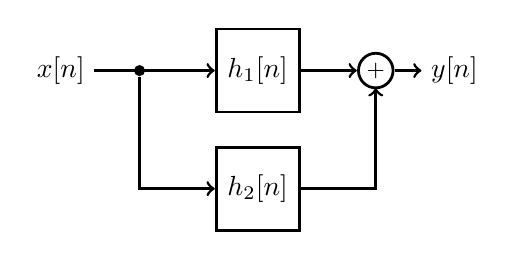
\begin{tikzpicture}
    \tikzstyle{block} = [draw, shape=rectangle, minimum height=3em, minimum width=3em, node distance=1.5cm, line width=1pt]
    \tikzstyle{sum} = [draw, shape=circle, node distance=1.5cm, line width=1pt, minimum width=1.25em]
    \tikzstyle{branch} = [fill,shape=circle,minimum size=4pt,inner sep=0pt]
    
    \node [left] at (0,0) (in) {$x[n]$};
    \node [branch, right of = in] (b1) {};
    \node [block, right of = b1] (h1) {$h_1[n]$};
    \node [block, below of = h1] (h2) {$h_2[n]$};
    \node [sum, right of = h1] (sum) {};
    \node at (sum) (plus) {\footnotesize$+$};
    \node [right of = plus] (out) {$y[n]$};
    
    \begin{scope}[line width=1pt]
    \draw [->] (in) -- (h1);
    \draw [->] (b1) |- (h2);
    \draw [->] (h2) -| (plus);
    \draw [->] (h1) -- (plus);
    \draw [->] (plus) -- (out);
    \end{scope}
\end{tikzpicture}
\vspace{1.5cm}

\plotsequence{{0/-1, 2/0, 0/1, 0/2, 0/3}}{$h_p[n]$}

\end{minipage}

Die Impulsantworten addieren sich. In diesem Fall werden die beiden IIR-Systeme zu einem FIR-System, da sich die Impulsantworten so überlagern, dass sich die unendlichen Reihen subtrahieren (Gut erkennbar mit Abbildung \ref{fig:g2} und \ref{fig:h2}, da $g_2[n] = h_1[n]$).
\end{aufgabe}

\begin{aufgabe}
	Das zeitdiskrete Signal $x[n]$ ist periodisch mit der ganzzahligen Periode $N$, wenn gilt:

$$x[n] = x[n+N]$$

Das kleinste $N$, das die Gleichung erfüllt, ist die gesuchte Grundperiode. Für trigonometrische Funktionen muss ebenfalls die Periodizität gelten.

$$\sin{(\varphi(n))} = \sin{(\varphi(n)+2\pi k)}\quad\cos{(\varphi(n))} = \cos{(\varphi(n)+2\pi k)}, \quad k \in \mathbb{Z}$$

\subsection*{(a)}

\begin{align*}
\cos{\left(\frac{30}{105}\pi(n+N)\right)} &\overset{!}{=} \cos{\left(\frac{30}{105}\pi n + 2\pi k\right)} &&\Bigg|\arccos \\
\frac{30}{105}\pi(n+N) &\overset{!}{=} \frac{30}{105}\pi \left(n+ 2k\cdot\frac{105}{30}\right) &&\Bigg| \frac{105}{30\pi} \ \Bigg| -n \\
N&\overset{!}{=} \frac{105}{15}k = 7k
\end{align*}

Das kleinste ganzzahlige Ergebnis liefert $k=1\implies N=7$. In den folgenden Rechnungen wird die Forderung direkt an das Argument der Winkelfunktion gestellt.

\begin{minipage}[t]{0.49\textwidth}

\subsection*{(b)}

\begin{align*}
    0.02\pi (n+N) &\overset{!}{=} 0.02\pi n + 2\pi k\\
    \frac{1}{50}\pi(n+N) &\overset{!}{=} \frac{1}{50}\pi (n+100k) \\
    N &\overset{!}{=} 100k \implies N = 100
\end{align*}

\end{minipage}
\begin{minipage}[t]{0.49\textwidth}

\subsection*{(c)}

\begin{align*}
5(n+N) &\overset{!}{=} 5n + 2\pi k \\
5n+5N &\overset{!}{=} 5n + 2\pi k \\
5N &\overset{!}{=} 2\pi k
\end{align*}
\centering
$\pi$ ist irrational, daher ist \\
das Signal nicht periodisch.
\end{minipage}

\newpage

\begin{minipage}[t]{0.49\textwidth}
\subsection*{(d)}

\begin{align*}
5\pi (n+N) &\overset{!}{=} 5\pi n + 2\pi k \\
5\pi n+ 5\pi N  &\overset{!}{=} 5\pi n + 2\pi k \\
5\pi N &\overset{!}{=} 2k\pi \\
N &\overset{!}{=} \frac{2}{5}k \implies N = 2
\end{align*}

\end{minipage}
\begin{minipage}[t]{0.49\textwidth}
\subsection*{(e)}

\begin{align*}
\frac{62}{10}\pi (n+N) &\overset{!}{=} \frac{62}{10}\pi n + 2\pi k \\
\frac{62}{10}\pi n+\frac{62}{10}\pi N &\overset{!}{=} \frac{62}{10}\pi n + 2\pi k \\
N&\overset{!}{=} \frac{20}{62} k = \frac{10}{31}k \implies N = 10
\end{align*}

\end{minipage}

\vspace{10pt}

Veranschaulicht durch \m{stem} Plots:

\begin{figure}[ht]
    \centering
    \includegraphics[width=0.7\linewidth]{images/Signals.png}
    \caption{Signale}
    \label{fig:sig}
\end{figure}
\end{aufgabe}

\begin{aufgabe}
	%%%%%%%%%%%%%%%%%%%%%%%%%%%%%%%%%%%%%%%%%%%%%%%%%%%%%%%%%%%%
%%                     Lösung Aufgabe 3                   %%
%%%%%%%%%%%%%%%%%%%%%%%%%%%%%%%%%%%%%%%%%%%%%%%%%%%%%%%%%%%%

\subsection{z-Transformation} \label{aufg:3a}

$$
H(z) = 1.2 + \frac{1}{2}\cdot\frac{z}{z+\frac{1}{2}} - \frac{3}{5} \frac{z}{z-\frac{1}{5}} = 1.2 + \frac{\frac{1}{2}}{1+\frac{1}{2}z^{-1}} -  \frac{\frac{3}{5}}{1-\frac{1}{5}z^{-1}}
$$

Kann mittels der Matlab-Funktion \m{residuez(r, p, k)} wie bereits in vorigen Übungen dokumentiert in Zähler- und Nennerpolynom umgerechnet werden.

$$
H(z) = \frac{1.1 - 0.04z^{-1} - 0.12 z^{-2}}{1 + 0.3z^{-1} - 0.1 z^{-2}}
$$

\newpage

%%%%%%%%%%%%%%%%%%%%%%%%%%%%%%%%%%%%%%%%%%%%%%%%%%%%%%%%%%%%

\subsection{Plot der Impulsantwort} \label{aufg:3b}

\begin{figure}[h]
\centering
\includegraphics[width=0.5\linewidth]{assets/A3b_h.png}
\end{figure}

%%%%%%%%%%%%%%%%%%%%%%%%%%%%%%%%%%%%%%%%%%%%%%%%%%%%%%%%%%%%

\subsection{Stabilität Prüfen} \label{aufg:3c}

\m{decomposeLTI} wirf zunächst keinen Fehler für Instabilität und liefert die Koeffizienten für die jeweiligen Anteile

\begin{itemize}
    \item[\textbf{Allpass:}]
    \m{b_all = [1, 0, 0]},
    
    \m{a_all = [1, 0, 0]}
    
    \item[\textbf{Min-Phase:}]
    \m{b_min = [1.0000, -0.0364, -0.1091]},
    
    \m{a_min = [1.0000    0.3000   -0.1000]}
\end{itemize}

Hier ist zu erkennen, dass die Koeffizienten beim Allpass-Anteil nur $a_0 = 1$ und $b_0 = 1$ sind. Bei einem solchen System ist der Phasengang konstant 0, was heißen muss, dass im Ursprüngliche System nur der Minimalphasenanteil auf die Phase wirkt. Das System ist also selbst ein Minimalphasensystem. Eine Alternative Begründung ist, dass alle ihre Null- (und Polstellen) innerhalb des Einheitskreises liegen.

\begin{figure}[h]
\begin{minipage}[t]{0.5\textwidth}
    \centering
    \includegraphics[width=0.7\linewidth]{assets/A3c_all.png}
    \caption{Phase des Allpass Anteil}
\end{minipage}
\begin{minipage}[t]{0.5\textwidth}
    \centering
    \includegraphics[width=0.7\linewidth]{assets/A3c_min.png}
    \caption{Phasengang des Minimalphasen Anteil gleich dem Phasengang des Gesamtsystems}
\end{minipage}
\end{figure}

\newpage

%%%%%%%%%%%%%%%%%%%%%%%%%%%%%%%%%%%%%%%%%%%%%%%%%%%%%%%%%%%%

\subsection{Plot der inversen Impulsantwort} \label{aufg:3d}

\begin{figure}[h]
\centering
\includegraphics[width=0.5\linewidth]{assets/A3d_hinv.png}
\end{figure}

%%%%%%%%%%%%%%%%%%%%%%%%%%%%%%%%%%%%%%%%%%%%%%%%%%%%%%%%%%%%

\subsection{Kaskadierung der Systeme} \label{aufg:3e}

\begin{figure}[h]
\centering
\includegraphics[width=0.5\linewidth]{assets/A3e_hcsc.png}
\end{figure}

Es bleibt nur ein Delta-Impuls als Resultierende Impulsantwort übrig.
\end{aufgabe}

%%%%%%%%%%%%%%%%%%%%%%%%%%%%%%%%%%%%%%%%%%%%%%%%%%%%%%%%%%%%%%%%%%%%%%%%%%%%%%%%

\appendix
\section*{Anhang}
\addcontentsline{toc}{section}{Anhang}

\crule{Z-Transformation}

\renewcommand{\arraystretch}{2.0} % Default value: 1
\renewcommand{\rm}{}

\begin{table}[h]
	\centering
	\caption{Rechensätze für kausale Signale} \label{tab:zt}
	\begin{tabularx}{\textwidth}{|c|
		>{$\displaystyle}Y<{$}
			>{$\displaystyle}c<{$}
		>{$\displaystyle}Y<{$}|}
		\hline
		1. & X(z) = \mathcal{Z}_n\{x[n]\}(z) & := & \sum\limits_{n=0}^{\infty} x[n] z^{-n} \\ [2.5ex] \hline \hline
		2. & \mathcal{Z}_n\{x[n-k]\}(z)      & =  & z^{-k}\mathcal{Z}_n\{x[n]\}(z)         \\ [2.5ex] \hline
	\end{tabularx}
\end{table}

\begin{table}[h]
	\centering
	\caption{z-Korrespondenztabelle} \label{tab:zkorr}
	\begin{tabularx}{\textwidth}{
		|c|
		>{$\displaystyle}Y<{$}
			>{$\displaystyle}c<{$}
		>{$\displaystyle}Y<{$}|
		}
		\hline
		1. & a^n u[n] & \ztransf & \quad \frac{z}{z-a} \\ [2.5ex] \hline
	\end{tabularx}
\end{table}
\renewcommand{\arraystretch}{1.0} % Default value: 1

\crule{Testsignale}

\begin{itemize}
	\item Kronecker Delta

	      \begin{minipage}{0.4\textwidth}\vspace*{0pt}
		      $$
			      \delta[n] = \begin{cases}
				      1 \text{ wenn } n=0 \\ 0 \text{ sonst}
			      \end{cases}
		      $$
	      \end{minipage}
	      \begin{minipage}{0.5\textwidth}\vspace*{0pt}
		      \centering
		      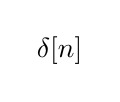
\begin{tikzpicture}[scale=0.7]
			      \node at (0, 2) {$\delta [n]$};
			      \ax{$n$}\nakedsequence{{0/-3, 0/-2, 0/-1, 1/0, 0/1, 0/2, 0/3}};
		      \end{tikzpicture}
	      \end{minipage}

	\item Sprungfunktion

	      \begin{minipage}{0.4\textwidth}\vspace*{0pt}
		      $$
			      u[n] = \begin{cases}
				      1 \text{ wenn } n\geq 0 \\ 0 \text{ sonst}
			      \end{cases}
		      $$
	      \end{minipage}
	      \begin{minipage}{0.5\textwidth}\vspace*{0pt}
		      \centering
		      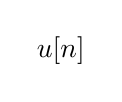
\begin{tikzpicture}[scale=0.7]
			      \node at (0, 2) {$u [n]$};
			      \ax{$n$}\nakedsequence{{0/-3, 0/-2, 0/-1, 1/0, 1/1, 1/2, 1/3}};
		      \end{tikzpicture}
	      \end{minipage}
\end{itemize}

\vspace{10px}

\crule{Potenzreihen}

\begin{itemize}
	\item  Logarithmus

	      \begin{equation}
		      \ln(1+x) = \sum_{n=1}^\infty (-1)^{n+1} \frac{x^n}{n}
		      \label{eq:potln}
	      \end{equation}

\end{itemize}

\bibliographystyle{plain}
\bibliography{assets/DanielCh}

\section*{Feedback}
\addcontentsline{toc}{section}{Feedback}

\begin{block}
	Durchgestrichenes Korrigiert
\end{block}

\begin{itemize}
	\item [1.d.] \sout{ROC beschrieben aber nicht eingezeichnet -0.25P}
\end{itemize}
%% 
%%%%%%%%%%%%%%%%%%%%%%%%%%%%%%%%%%%%%%%%%%%%%%%%%%%%%%%%%%%%%%%%%%%%%%%%%%%%%%%%

\cleardoubleoddpage

\end{document}
\endinput
